% !TEX root = ../../../main.tex
% 来源：中学数学实验教材·第二册（几何）
% 章节：实验几何 / 方向、角度与平行
% 原始文件：1.tex，行 1333-1357
% 类型：tikz
% ---
\begin{tikzpicture}[>=latex]
\begin{scope}
\tkzDefPoints{2/0/A, 0/0/O}
\tkzDefPoint(30:1.8){B1}
\tkzDrawSegments(A,O B1,O)
\tkzMarkAngles[mark=none, size=.6](A,O,B1)
\tkzLabelAngle[pos=.8](A,O,B1){$\alpha$}
\end{scope}
\begin{scope}[xshift=4cm]
	\tkzDefPoints{2/0/A, 0/0/O}
\tkzDefPoint(60:1.8){B2}
\tkzDrawSegments(A,O B2,O)
\tkzMarkAngles[mark=none, size=.6](A,O,B2)
\tkzLabelAngle[pos=.8](A,O,B2){$\beta$}
\end{scope}
\begin{scope}[xshift=8cm]
	\tkzDefPoints{2/0/A, 0/0/O, 0/2/C}
\tkzDefPoint(30:1.8){B1}
\tkzDrawSegments(A,O B1,O O,C)
\tkzMarkAngles[mark=none, size=.6](A,O,B1)
\tkzLabelAngle[pos=.8](A,O,B1){$\alpha$}
\tkzMarkAngles[mark=none, size=.5](B1,O,C)
\tkzLabelAngle[pos=.8](B1,O,C){$\beta$}
\end{scope}
\end{tikzpicture}
